\documentclass[a4paper, 11pt]{article}
\usepackage[pdftex]{graphicx}
\usepackage{parskip}
\usepackage{hyperref}
\usepackage[all]{hypcap}
\usepackage{amsmath}
\usepackage{amsfonts}
\usepackage{xcolor}
\usepackage{enumitem}
\title{Assignment 3 -- Math 205 Linear Algebra}
\author{Syed Ammar Mahdi \\sm03691 \and Muhammad Shahzain \\ms03977 \and Muhammad Shahrom Ali \\ma03559}

\newcommand{\mat}[1]{\boldsymbol { \mathsf{#1}} }
\newcommand{\MYhref}[3][blue]{\href{#2}{\color{#1}{#3}}}


\begin{document}
\setlength{\parskip}{10pt} % 1ex plus 0.5ex minus 0.2ex}
\setlength{\parindent}{0pt}
\DeclareGraphicsExtensions{.pdf,.png,.gif,.jpg}
\maketitle

\section*{Solutions}
\begin{enumerate} 

\item Does the following set of polynomials constitute a basis for subspace of polynomial of degree less than equal to 2 \[
\left\{x^2 + x + 1, x^2 - x + 1, 2x^2, 1 \right\}
\]

\item Find a basis for the space of polynomials $p(x)$ of degree $\leq 2$? Then, find the basis for the subspace with $p(7) = 0$ and sketch the bases.

\item Let $P_3$ be the real number vector space over $\mathbb R$ of cubic polynomials. $W$ is defined as \[
W = \{p(x) \in P_3 \;|\; p'(-1) = 0 \;\; \text{and} \;\; p''(1) = 0\}
\]

Determine whether $W$ forms a subspace of $V$

\item Find the bases for the four subspaces associated with $\mat A$ and $\mat B$:
\[ A = \left[ \begin{array}{ccc}
1&2&4\\
2&4&8
\end{array} \right]
\hspace{10mm}, B = \left[ \begin{array}{ccc}
1&2&4\\
2&5&8
\end{array} \right]\]
Sketch the four subspaces if an arbitrary matrix $\mat C$ is \begin{itemize}
  \item invertible
  \item a zero matrix
\end{itemize}

\item Find the complete solution for the following equations and describe the solution space:
\begin{equation} \label{eq1}
\begin{split}
x + 3y + 3z = 1\\
2x + 6y + 9z = 5\\
-x - 3y +3z =5.
\end{split}
\end{equation}

\item You are given an equilateral triangle whose sides are of unit length. You are given a complex function $f(\eta_1, \eta_2)$ which transforms the equilateral triangle as shown in the following figure (left and middle). We can then copy and rotate the transformed triangle to form a complete patch as shown in the following figure on the right. Note that we don't have any duplicate points on the final patch 
\begin{center}
  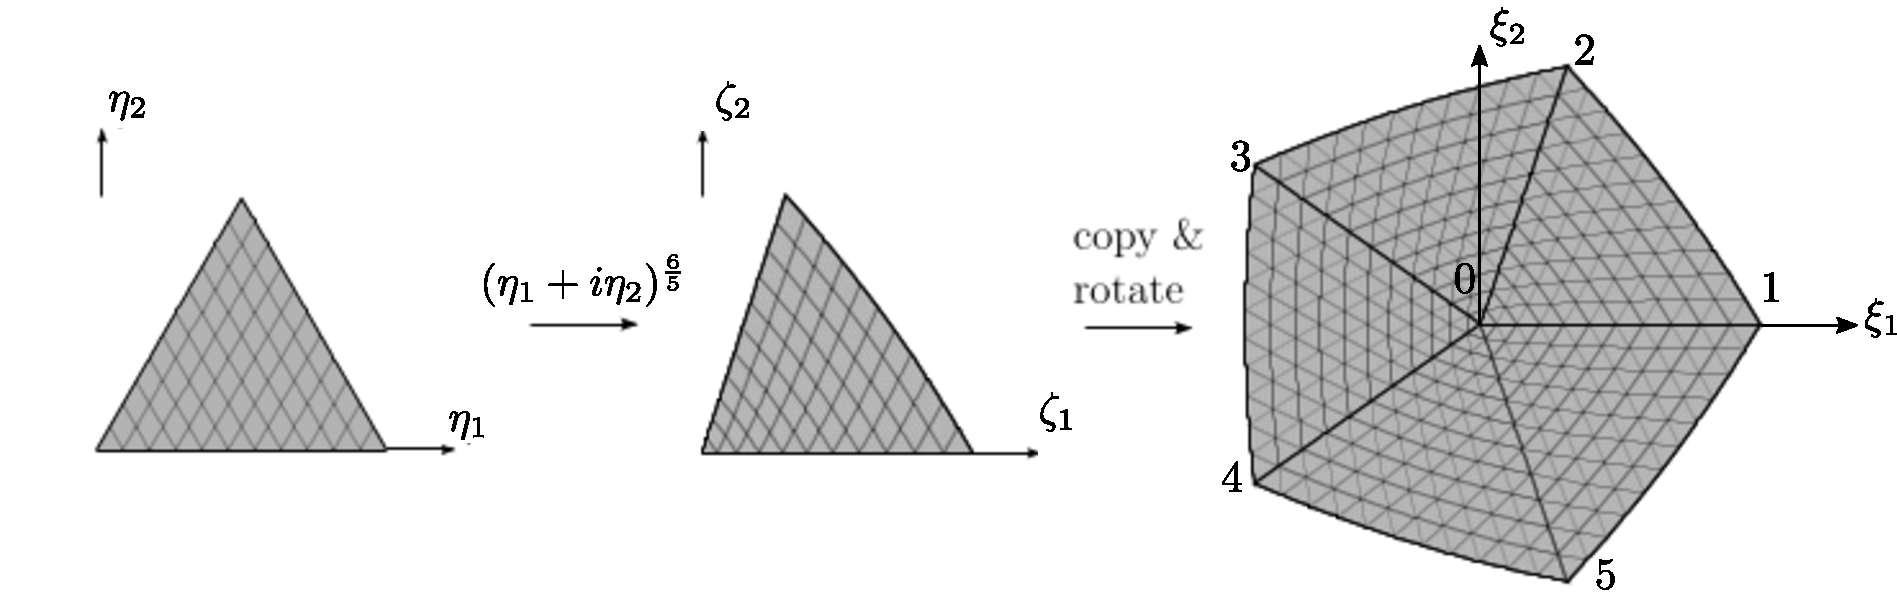
\includegraphics[scale=0.4]{figs/q1.pdf}
\end{center}
\begin{enumerate}[label=(\alph*)]
\item Calculate the coordinates of the 6 points on the patch.
\item An engineer measured the charge distrbution $q$ on the 6 points of the patch as follows:
    \begin{center}
    \begin{tabular}{ | l | l | l | l | l | l | l |}
    \hline
    Point \# & 0 & 1 & 2 & 3 & 4 & 5  \\ \hline
    q        & 1 & 3 & 1 & 0 & 1 & 2 \\ \hline
    \end{tabular}
    \end{center}
    An electrical engineer is interested in finding out the charge $q$ at $\vec \xi = (0.5, 0.5)^T$. He also tells you that the charge inside the patch can be approximated using a bilinear polynomial $(1, \xi_1, \xi_2,\xi_1\xi_2)$. Compute $q$ at $\vec \xi = (0.5, 0.5)^T$. 
    \item Sketch the charge distribution surface over the $\xi_1 - \xi_2$ patch.
\end{enumerate}

\item We have learned that for underdetermined systems, it is impossible to find unique solutions in the absence of some extra constraints. One way of obtaining the unique solution is to impose a minimum $L_2$ norm constraint i.e.
\begin{align}
\text{Solve: } \;\; \mat A \vec x &= \vec b \\
\text{such that: } \;\; \|\vec x\|_2 &\;\; \text{is minimum}
\end{align}
In this case, $\vec x_r = \mat A^T (\mat A \mat A^T)^{-1} \vec b$. By way of example explain the relationship between $\vec x_p$ and $\vec x_n$, and when $\vec x_p = \vec x_r$. Sketch the four fundamental subspaces

\item Explain, with reason, whether the following statements are true or false
\begin{enumerate}[label=(\alph*)]
\item The complete solution is any linear combination of $x_p$ and $x_n$
\item A system $\mat A \vec x = \vec b$ has at most one particular solution
\item The solution $x_p$ with all free variables set to zero can be the shortest solution (minimum length $\|x\|$)
\item If $\mat A$ is invertible there is no solution $x_n$ in the nullspace
\end{enumerate}

\item True or false (with a reason or a counterexample)
\begin{enumerate}[label=(\alph*)]
\item $\mat A$ and $\mat A^T$ have the same number of pivots
\item $\mat A$ and $\mat A^T$ have the same left nullspace
\item If the row space equals the column space then $\mat A = \mat A^T$
\item If $-\mat A = \mat A^T$, then the row space of $\mat A$ equals the column space  
\end{enumerate}


\item For the space $\mathbb R^4$, let $w_1 = \begin{bmatrix} 1 \\ 1 \\ 1 \\ 1\end{bmatrix}, w_2 = \begin{bmatrix} 3 \\ 3 \\ -1 \\ -1\end{bmatrix}, y = \begin{bmatrix} 6 \\ 0 \\ 2 \\ 0\end{bmatrix}$, and let $W = \text{sp}\{w_1, w_2\}$. 

\begin{enumerate}[label=(\alph*)]
\item Find a basis for $W$ consisting of two orthogonal vectors using Gram-Schmidt process.
\item Explain the Gram-Schmidt process intuitively. 
\item Express $y$ as the sum of a vector in $W$ and a vector in $W^\perp$
\end{enumerate}

Please refer to \MYhref{https://textbooks.math.gatech.edu/ila/orthogonal-sets.html}{this link} for this question

\end{enumerate}
\end{document}